\begin{figure}
    \centering
    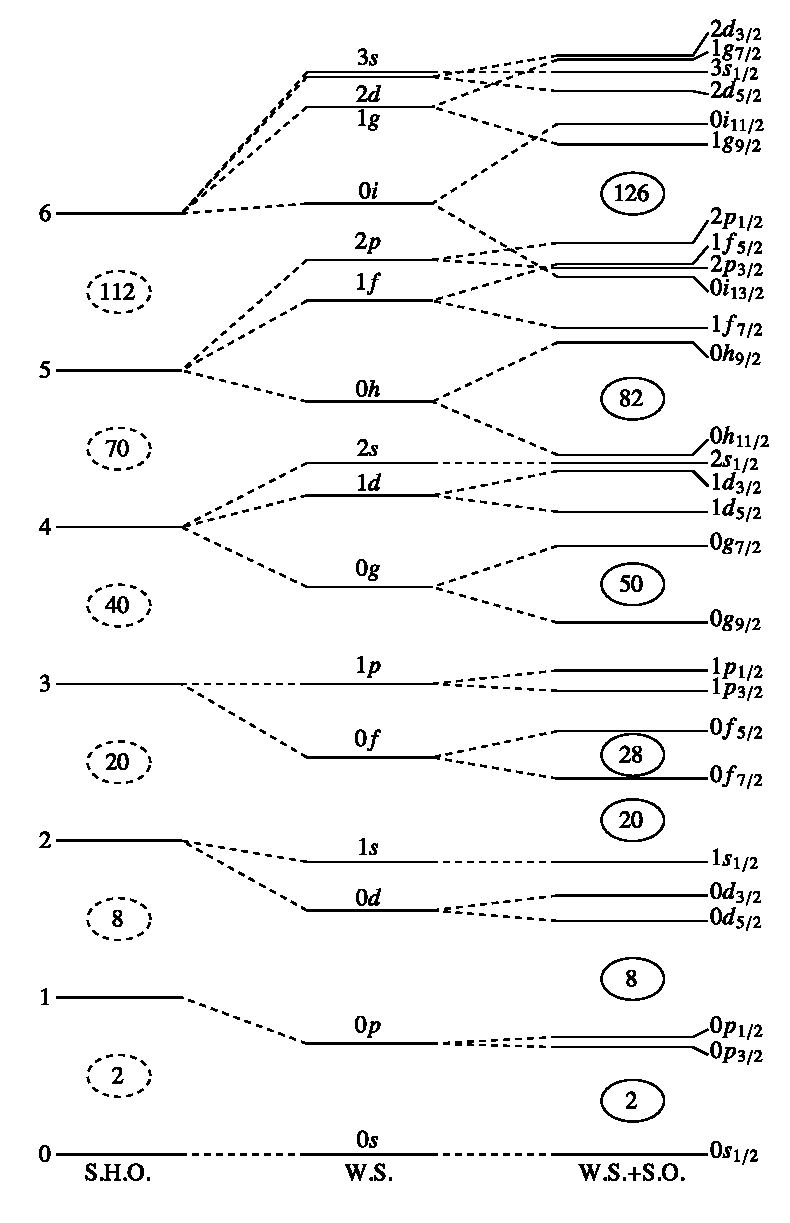
\includegraphics[scale=0.8]{Introduction_Figs/Shellmodel.eps}
    \caption{The evolution of the shell model and the creation of the closed shells of a spherical nucleus. On the left is the spherical harmonic oscillator. By changing the potential to the Woods-Saxon potential, creating a flat centered potential well, the degenerate states of the harmonic oscillator separate in energy. By further adding a spin-coupling term, the levels separate with energy spacings that create the closed shells and the magic numbers.}
    \label{fig:shellmodel}
\end{figure}